\documentclass{beamer}
\usepackage[T1]{fontenc}
\usepackage[utf8]{inputenc}
\usepackage{lmodern}
\usepackage[francais]{babel}
\usepackage{graphicx}
\usepackage{beamerthemeWarsaw}
\expandafter\def\expandafter\insertshorttitle\expandafter{\insertshorttitle\hfill\insertframenumber\,/\,\inserttotalframenumber}

\title{Algorithmes distribués sur Android}
\author{Kevin \textsc{Boulala}, Maxime \textsc{Dubois}}
\institute{Université de Franche Comté}
\date{4 février 2016}

\begin{document}

  \begin{frame}
    \titlepage
  \end{frame}

  \begin{frame}
    \setcounter{tocdepth}{1}
    \tableofcontents[]
  \end{frame}
  
  \section{Présentation générale}
  \begin{frame}
    \frametitle{Présentation générale}
    \begin{block}{L'objectif principal}
      Développement d'une plateforme permettant de programmer simplement des algorithmes distribués et de les exécuter sur des appareils android.
    \end{block}
    \begin{block}{Les autres objectifs}
      \begin{itemize}
        \item Utiliser cette plateforme pour implanter des algorithmes distribués
        \item Développer une application utilisant ces algorithmes distribués
      \end{itemize}
    \end{block}
  \end{frame}
  
  \section{Choix technologiques}
  \begin{frame}
    \setcounter{tocdepth}{2}
    \tableofcontents[currentsection]
  \end{frame}
    \subsection{Les options}
    \begin{frame}
      \frametitle{Choix technologiques}
      \framesubtitle{Les options}
      \begin{small}
        \begin{block}{NFC}
          \begin{itemize}
            \item Android compatible depuis la version Ice Cream Sandwich (4.0)
            \item Connexion des appareils très facile
          \end{itemize}
        \end{block}
        \begin{block}{Bluetooth}
          \begin{itemize}
            \item Quelques chiffres : création en 1994, > 28000 membres
            \item Utilisé pour les communications, le transfert de fichiers
          \end{itemize}
        \end{block}
        \begin{block}{Wi-Fi Direct}
          \begin{itemize}
            \item Wi-Fi mais sans point d'accès intermédiaire
            \item Pour la même utilisation que le Bluetooth pour les appareils Android
          \end{itemize}
        \end{block}
      \end{small}
    \end{frame}
    \subsection{Bilan}
    \begin{frame}
      \frametitle{Choix technologiques}
      \framesubtitle{Bilan}
      \begin{small}
        \begin{block}{Synthèse des technologies}
          \begin{table}
            \begin{center}
              \begin{tabular}{|c|c|c|c|}
                \hline
                & \textbf{NFC} & \textbf{Bluetooth} & \textbf{Wi-Fi Direct} \\
                \hline
                \textbf{Vitesse (en Mbit/s)} & 0,424 & 24 & 250 \\
                \hline
                \textbf{Portée (en m)} & 0,1 & 10 & 60 \\
                \hline
              \end{tabular}
            \end{center}
          \end{table}
        \end{block}
        \begin{block}{Solution retenue}
          \begin{itemize}
            \item Wi-Fi Direct nécessite que l'utilisateur valide chaque connexion
            \item Quelques instabilités avec le Wi-Fi Direct et nos appareils
          \end{itemize}
          \begin{center}
            $ \Rightarrow $ Pour ces raisons, nous avons retenu le \textbf{Bluetooth}.
          \end{center}
        \end{block}
      \end{small}
    \end{frame}
  
  \section{Construction du réseau}
  \begin{frame}
    \setcounter{tocdepth}{2}
    \tableofcontents[currentsection]
  \end{frame}
    \subsection{Les objectifs}
    \begin{frame}
      \frametitle{Construction du réseau}
      \framesubtitle{Les objectifs}
      \begin{small}
        \begin{block}{Les objectifs}
          \begin{itemize}
            \item Connexions automatiques
            \item Ignorer les appareils qui ne nous intéressent pas
          \end{itemize}
          $ \Rightarrow $ Pas de topologie classique des réseaux Bluetooth (maître - esclaves)
          \begin{columns}
            \begin{column}{.5\textwidth}
              \begin{figure}
                \begin{center}
                  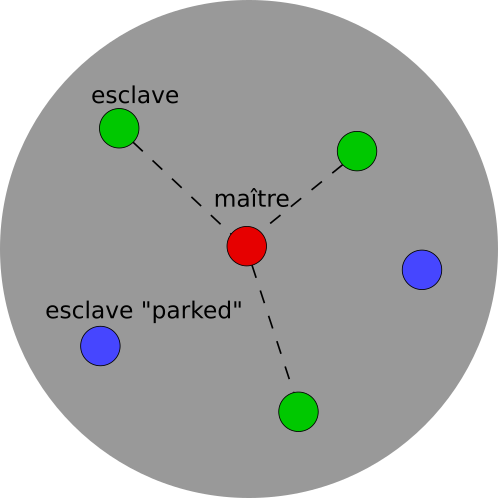
\includegraphics[width=.4\textwidth]{images/BluetoothPiconet.png}
                  \label{fig:piconet}
                  \caption{Un piconet}
                \end{center}
              \end{figure}
            \end{column}
            \begin{column}{.5\textwidth}
              \begin{figure}
                \begin{center}
                  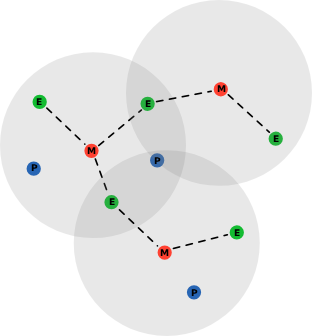
\includegraphics[width=.4\textwidth]{images/BluetoothScatternet.png}
                  \label{fig:scatternet}
                  \caption{Un scatternet}
                \end{center}
              \end{figure}
            \end{column}
          \end{columns}
        \end{block}
      \end{small}
    \end{frame}
    \begin{frame}
      \frametitle{Construction du réseau}
      \framesubtitle{Les objectifs}
      \begin{block}{Pas de maître, ni d'esclave}
        \begin{figure}
          \begin{center}
            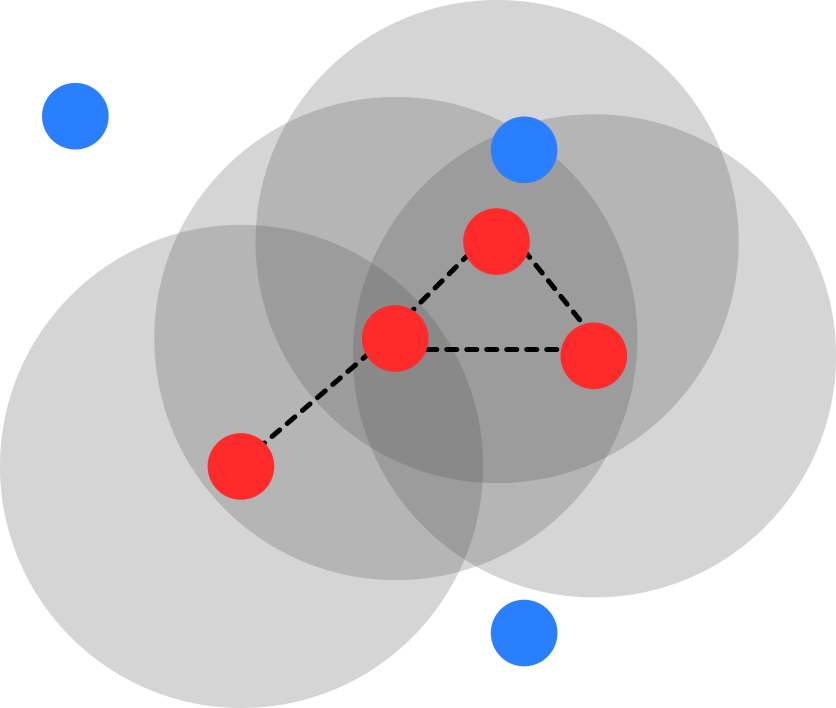
\includegraphics[width=.4\textwidth]{images/reseau_quelconque.png}
            \caption{Un réseau quelconque}
            \label{fig:quelconque}
          \end{center}
        \end{figure}
      \end{block}
    \end{frame}
    \subsection{Connexion automatique}
    \begin{frame}
      \frametitle{Connexion automatique}
      \framesubtitle{Identification et adressage}
      \begin{block}{Adresse MAC}
        \begin{itemize}
          \item Bluetooth est un protocole réseau n'utilisant pas IP
          \item Bluetooth utilise des adresses MAC
          \item Pour identifier les appareils, nous utilisons nous aussi les adresses MAC
        \end{itemize}
      \end{block}
    \end{frame}
    \begin{frame}
      \frametitle{Connexion automatique}
      \framesubtitle{Les socket bluetooth dans Android}
      \begin{block}{Les comportements}
        \begin{itemize}
          \item Les données transférées restent intactes ou les erreurs sont détectées
          \item Les données transférées arrivent dans le même ordre dans lequel elles ont été envoyés
        \end{itemize}
      \end{block}
      \begin{block}{Mode de connexion : secure ou insecure}
        \begin{itemize}
          \item « insecure » ne demande pas de confirmation à l'utilisateur contrairement à « secure »
          \item Une fois la connexion établit, les échanges sont chiffrés dans les deux modes
        \end{itemize}
      \end{block}
    \end{frame}
    \begin{frame}
      \frametitle{Connexion automatique}
      \framesubtitle{Les socket bluetooth dans Android}
      \begin{block}{Les problèmes}
        \begin{itemize}
          \item Ne peut faire du multi-client éfficacement et simplement \\
          $ \Rightarrow $ Un thread de réception, un thread d'envoi
          \item Les exceptions sont toutes du type IOException \\
          $ \Rightarrow $ Il faut alors analyser le message de l'exception
        \end{itemize}
      \end{block}
    \end{frame}
    \begin{frame}
      \frametitle{Connexion automatique}
      \framesubtitle{Rendre l'appareil visible}
      \begin{block}{La solution classique}
        L'API Android propose une solution pour rendre un appareil découvrable.
        \begin{itemize}
          \item Nécessite la validation manuelle de l'utilisateur
          \item Ne dure qu'un certain temps
        \end{itemize}
      \end{block}
      \begin{block}{Notre solution}
        Nous utilisons l'introspection de Java pour accéder à une API cachée et appeler la méthode setScanMode qui supprime les limitations de la solution classique. Mais...
        \begin{itemize}
          \item aucune assurance que cette méthode reste viable dans les prochaines versions d'Android
        \end{itemize}
      \end{block}
    \end{frame}
    \begin{frame}
      \frametitle{Connexion automatique}
      \framesubtitle{Détecter des appareils}
      \begin{block}{Détection}
        L'API Android fournit une méthode startDiscovery() qui lance une recherche pendant 12 secondes. Nous remarquons cependant que cette découverte est coûteuse :
        \begin{itemize}
          \item consomme de l'énergie
          \item sollicite beaucoup le bluetooth rendant le tout instable (peut provoquer des déconnexions)
        \end{itemize}
        Il faut donc utiliser cette fonctionnalité judicieusement.
      \end{block}
    \end{frame}
    \begin{frame}
      \frametitle{Connexion automatique}
      \framesubtitle{Comment se connecter aux bons appareils ?}
      \begin{block}{Récupération des UUIDs d'un appareil}
        \begin{itemize}
          \item UUID : Universal Unique Identifier
          \item Permet l'identification des services
          \item Mais
          \begin{itemize}
            \item la liste des UUIDs récupérés étaient souvent incomplètes ou vides
            \item le mécanisme coûteux en bande passante
          \end{itemize}
        \end{itemize}
        \begin{center}
          $ \Rightarrow $ On a donc abandonné cette solution
        \end{center}
      \end{block}
    \end{frame}
    \begin{frame}
      \frametitle{Connexion automatique}
      \framesubtitle{Comment se connecter aux bons appareils ?}
      \begin{block}{Solution de remplacement de la récupération des UUIDs}
        \begin{itemize}
          \item On ne cherche plus à savoir si un périphérique possède une UUID précise
          \item L'application se connecte directement et on attend un timeout
        \end{itemize}
      \end{block}
    \end{frame}
    \subsection{Solution proposée}
    \begin{frame}
      \frametitle{La solution proposée}
      \framesubtitle{}
      \begin{block}{Stabilisation du réseau}
        \begin{itemize}
          \item Lancer une seule découverte par périphérique lors du démarrage de l'application
          \item Limité à 4 connexions pour s'assurer une certaine stabilité
        \end{itemize}
      \end{block}
      \begin{block}{Problème}
        \begin{itemize}
          \item Lorsqu'un périphérique se déconnecte, le réseau peut s'éffondrer aléatoirement
        \end{itemize}
      \end{block}
    \end{frame}
    \begin{frame}
      \frametitle{La solution proposée}
      \framesubtitle{}
      \begin{block}{Réseau en forme d'arbre}
        \begin{figure}
          \begin{center}
            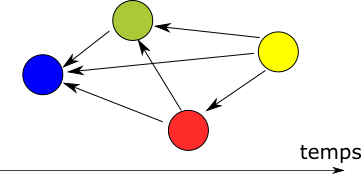
\includegraphics[width=.5\textwidth]{images/auto.png}
            \caption{Exemple de réseau}
            \label{fig:auto}
          \end{center}
        \end{figure}
      \end{block}
    \end{frame}

  \section{Routage}
  \begin{frame}
    \frametitle{Routage}
    \framesubtitle{}
  
  \end{frame}
  
  \section{API}
  \begin{frame}
    \frametitle{API}
    \framesubtitle{}
  	\begin{block}{Finalité}
        \begin{itemize}
        	\item Permettre une utilisation simple et efficace des mécanismes de connexions automatiques et de routage.
        \end{itemize}
    \end{block}
    \begin{block}{Comment ?}
    \begin{itemize}
    	\item Service Android.
    \end{itemize}
    \end{block}
  \end{frame}
    \begin{frame}
    \frametitle{API}
    \framesubtitle{Service Android}
  	\begin{block}{Qu'est-ce que c'est ?}
        \begin{itemize}
        	\item Un mécanisme propre à Android pour executer une tache en dehors de l'application
        	\item Propose des mécanismes de communications bidirectionnels entre une application et le service.
        \end{itemize}
    \end{block}
  \end{frame}
  \begin{frame}
    \frametitle{API}
    \framesubtitle{}
        \begin{figure}
          \begin{center}
            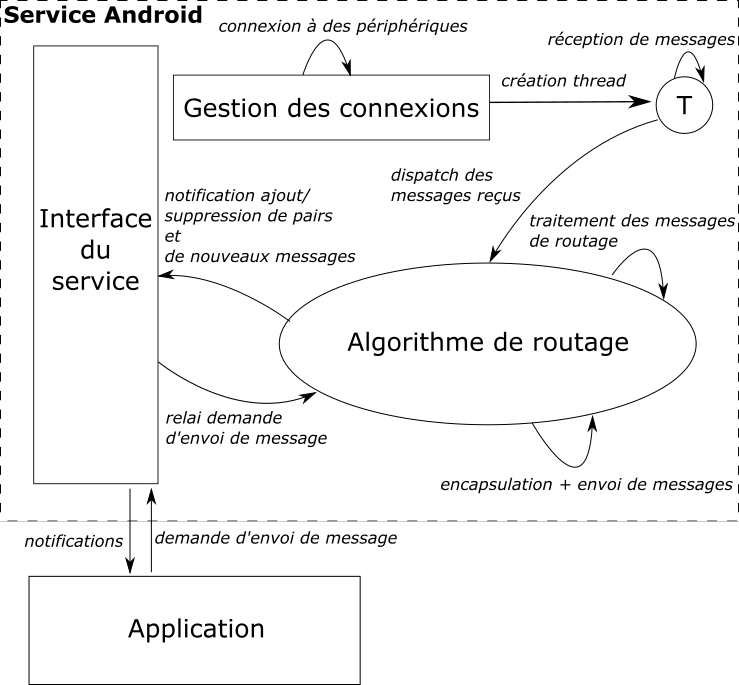
\includegraphics[width=.6\textwidth]{images/api.png}
            \label{fig:auto}
          \end{center}
        \end{figure}
  \end{frame}
  
  % TODO La suite dépend de ce qu'on aura produit d'ici jeudi.
  
  \section{Bilan}
  \begin{frame}
    \frametitle{Bilan}
    \framesubtitle{}
  
  \end{frame}
  
\end{document}
